We are now ready to describe the results of our experiments. Next few sections parallel the examples in section~\ref{sec-examples} and contain problem-specific details about algorithm~\ref{algo:steady} e.g. $\Omega_I, E$ etc. All computations were done with float32 numbers.
\subsection{2D ring system}Figure~\ref{fig:2D-surface} shows the learned and true solutions for the 2D ring system. Note that algorithm~\ref{algo:steady} produces an unnormalized zero of $\mathcal L$ but on the left panel the learned solution has been normalized for easier visualization. 
\begin{figure}[!ht]
    \centering
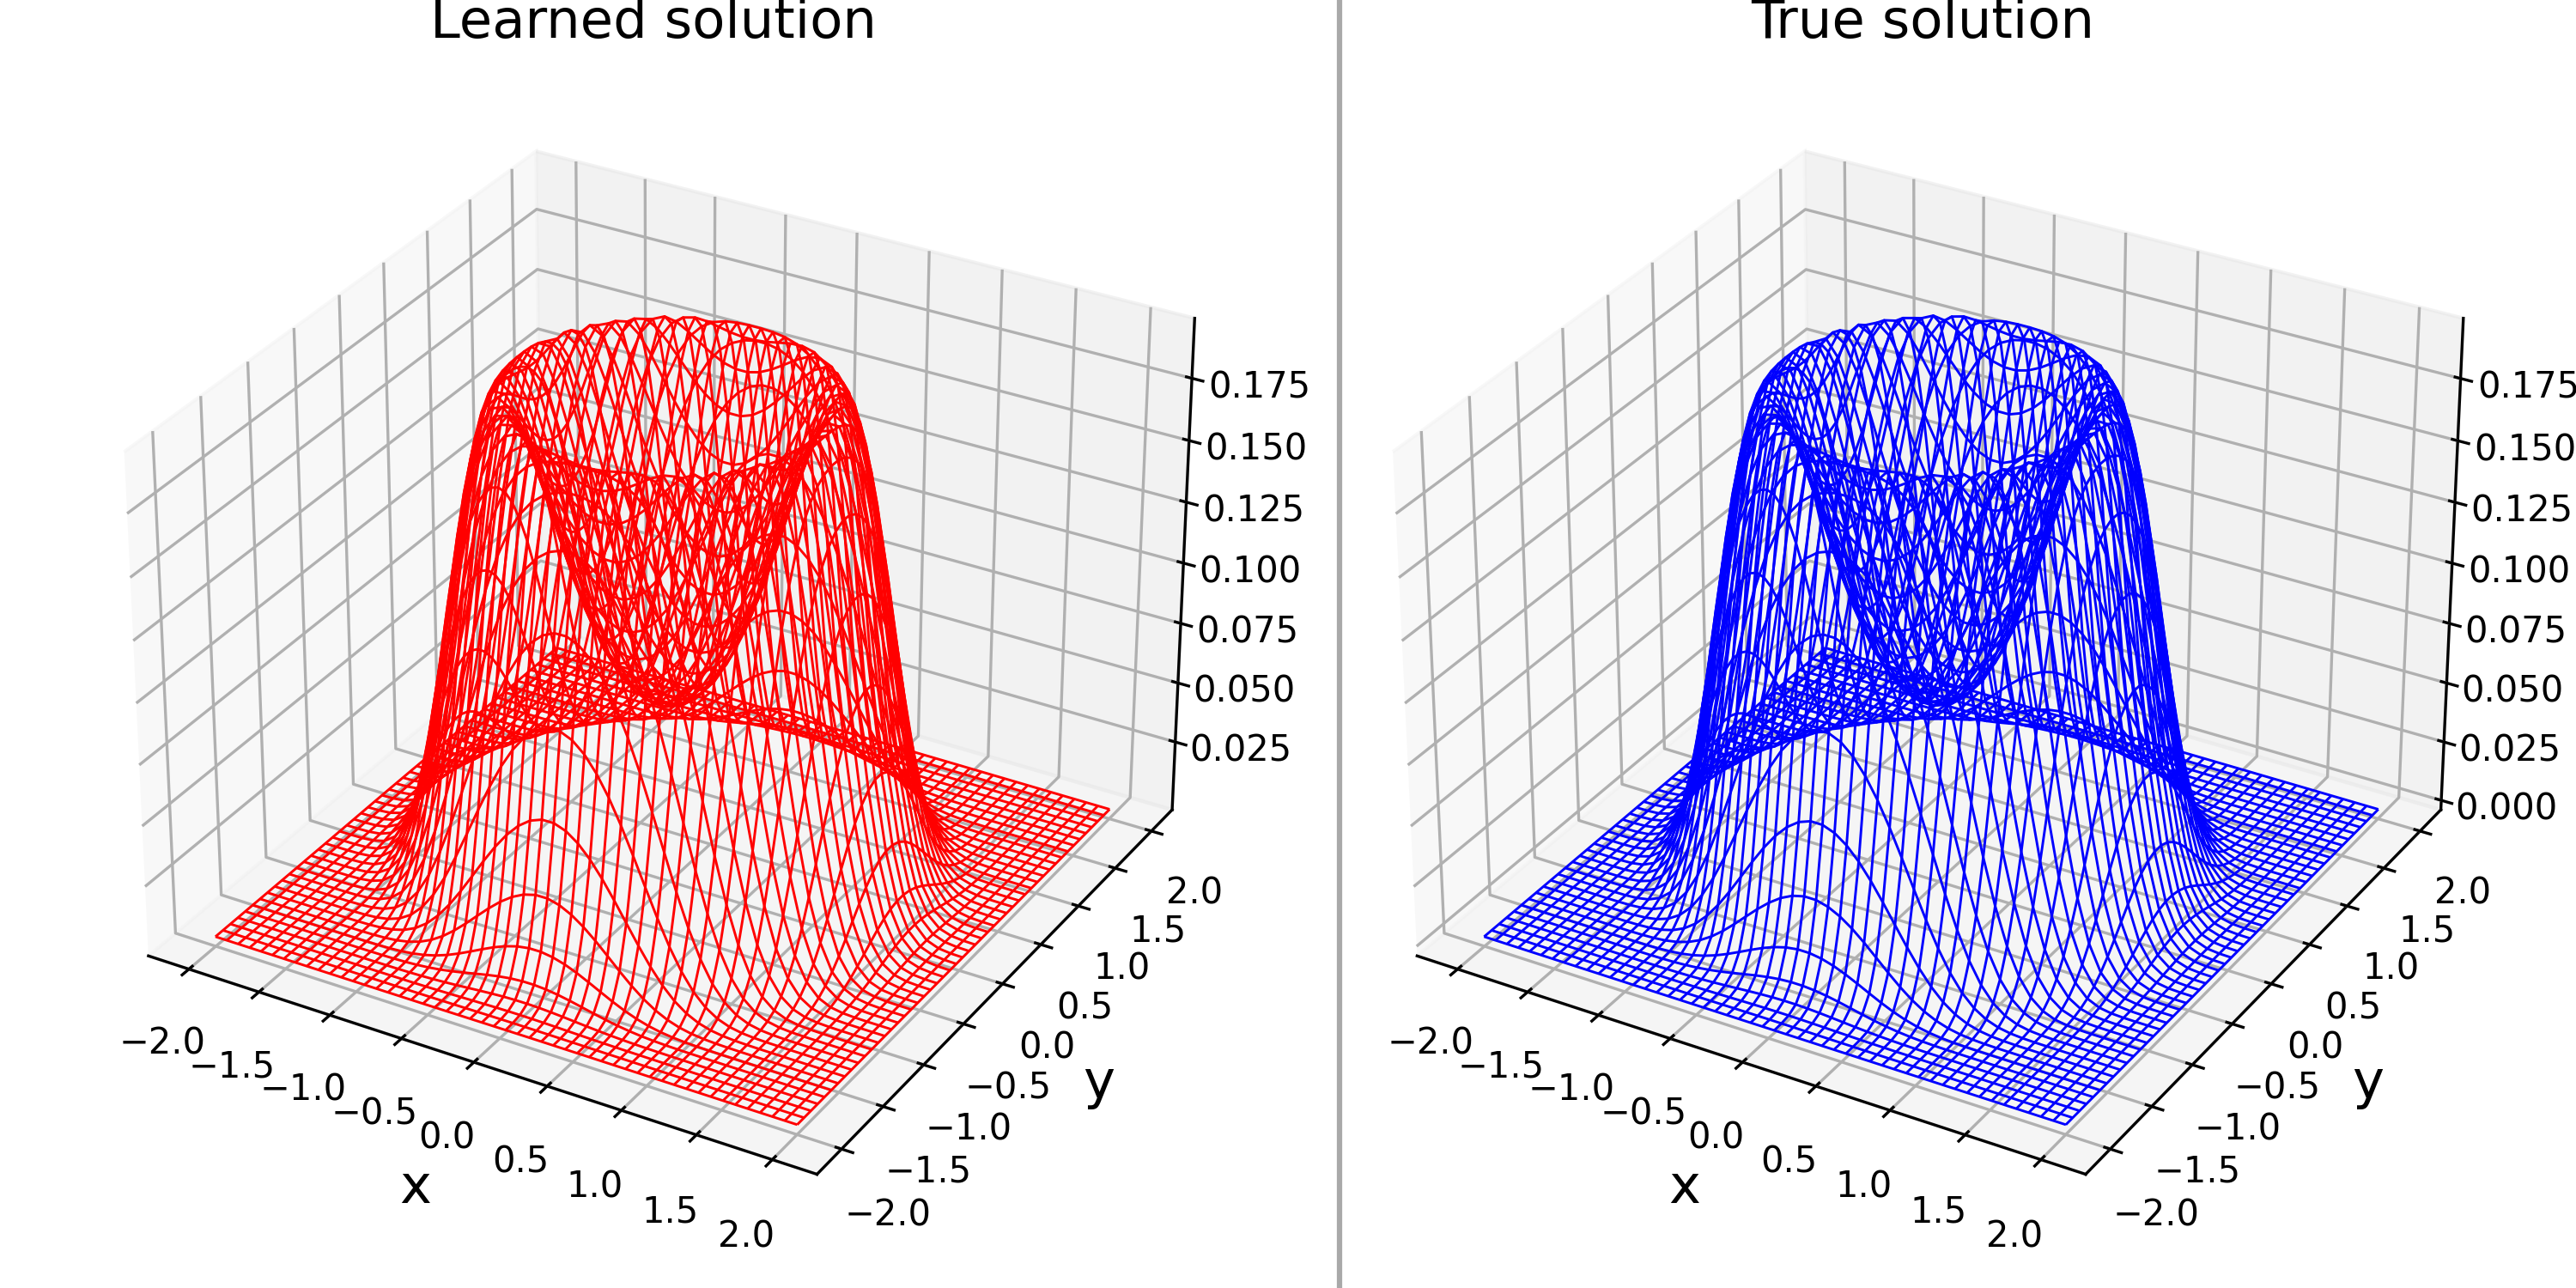
\includegraphics[scale=0.6
]{steady-plots/2D-surface.png}
    \caption{Solution for the 2D ring system}
    \label{fig:2D-surface}
\end{figure}
In this case we use $\Omega_I=[-2,2]^2$ and $E=8\times10^5$ iterations. 
\subsubsection{Comparison with Monte Carlo}\label{sssec-MC-comparison} Since the network was trained with domain resampling every $10$ steps and a mini-batch size of $N=1000$, during the entire training procedure $8\times10^7$ points were sampled from the domain. We compute the steady state with Monte Carlo with $8\times10^7$ particles to compare errors produced by both methods. Here the SDE trajectories were generated till time 10 with time-steps of 0.01. Since in this case we know the analytic solution we can compute and compare absolute errors. As we can see in figure~\ref{fig:MC-comparison}, for the same number of overall sampled points, Monte Carlo error is an order of magnitude larger than deep learning error. 

\begin{figure}[!ht]
    \centering
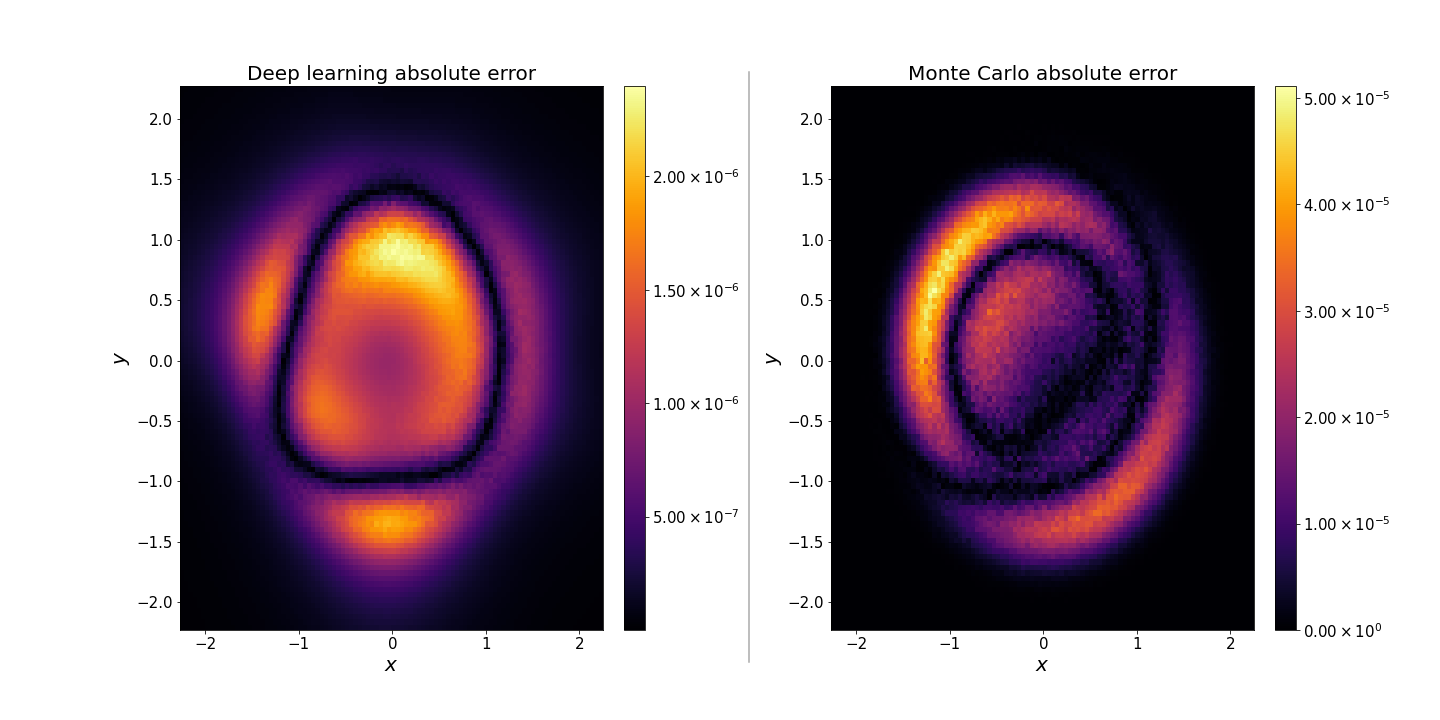
\includegraphics[scale=0.32]{steady-plots/2D-error.png}
\caption{Comparison of absolute errors for deep learning and Monte Carlo solutions for the 2D ring system}
    \label{fig:MC-comparison}
\end{figure}

\subsection{2nD ring system}
Although we solve this system for $n=1,2,3,4,5$, in this section we only produce the results for $n=5$ or $d=10$ to avoid repetition. Figure~\ref{fig:10D-surface} shows the solutions for  the 10D ring system for $\Omega_I=[-2, 2]^{10}$ and $E=4.6\times10^6$. In order to visualize the solution we focus on the quantity
$
    p(0, 0, 0, 0, x_4, x_5, 0, 0, 0, 0)
$.
For a visual comparison with the true solution normalization is desirable. But rather than trying to compute a 10-dimensional integral which is a non-trivial problem in itself we can normalize $
    p(0, 0, 0, 0, x_4, x_5, 0, 0, 0, 0)
$ which is much easier to do and due to the decoupled nature of this problem we can expect an identical result as in figure~\ref{fig:2D-surface} which is what we see in figure~\ref{fig:10D-surface}. In both of the panels the solutions have been normalized in a way such that,
$$\int_{\mathbb R}\int_{\mathbb R}p(0, 0, 0, 0, x_4, x_5, 0, 0, 0, 0)\,dx_4\,dx_5=1$$

\begin{figure}[!ht]
    \centering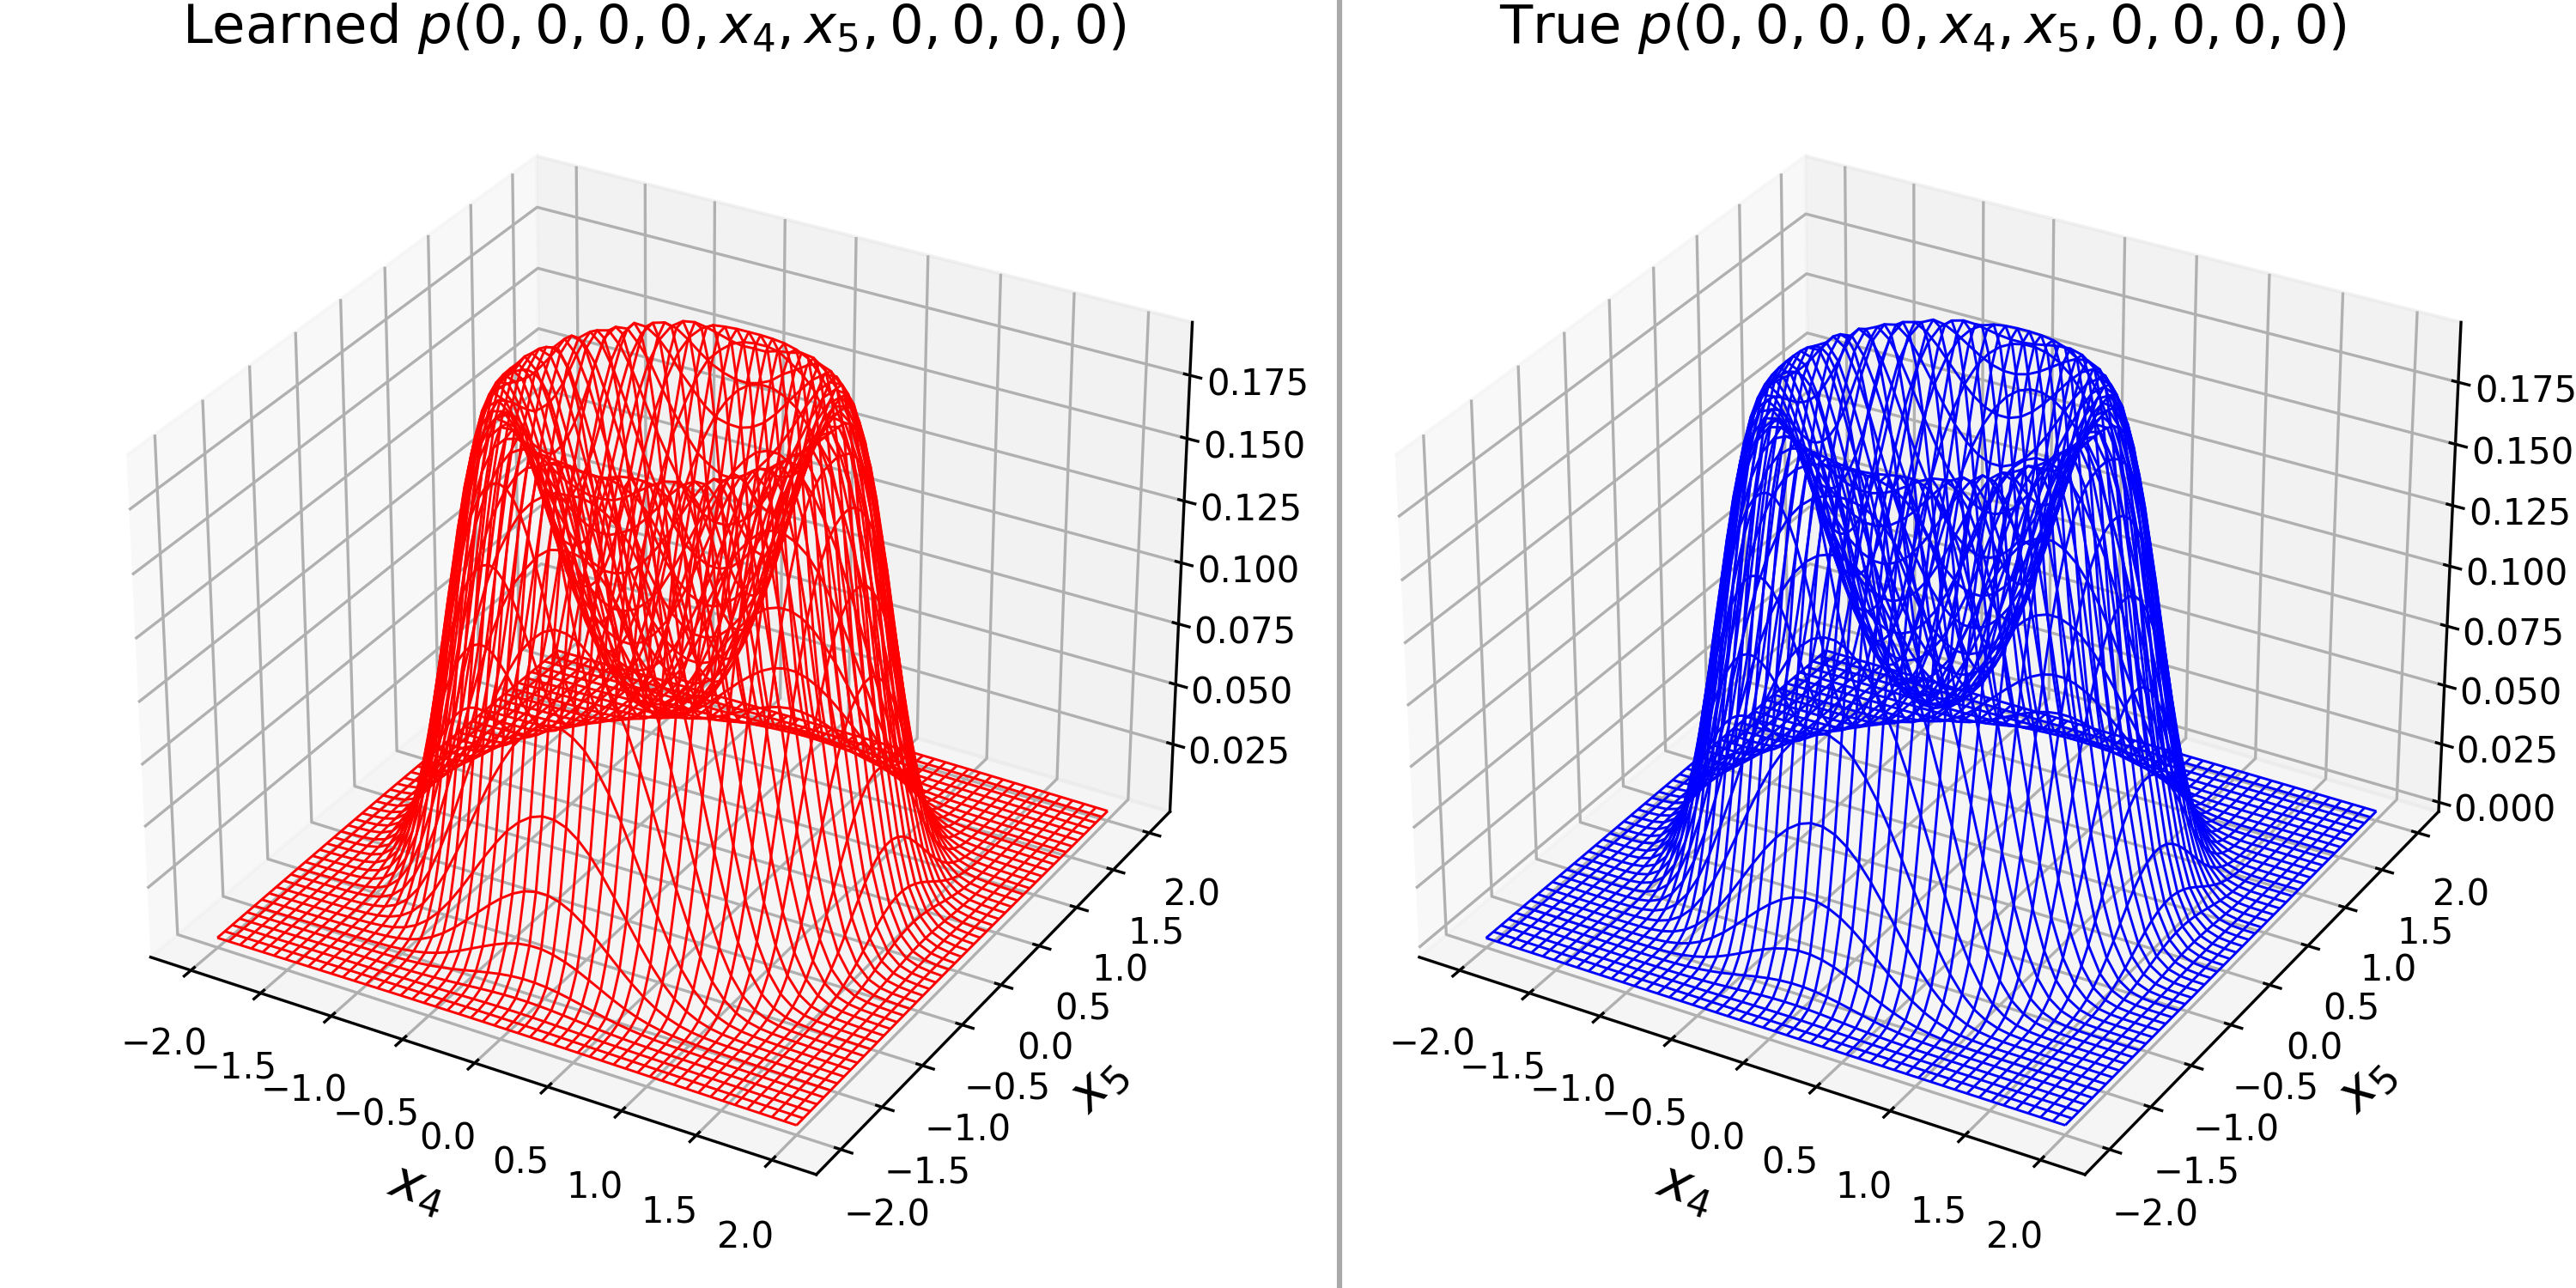
\includegraphics[scale=0.6
]{steady-plots/10D-surface.png}
\caption{Solutions for the 10D ring system. Both solutions have been normalized such that $\int_{\mathbb R}\int_{\mathbb R}p(0, 0, 0, 0, x_4, x_5, 0, 0, 0, 0)\,dx_4\,dx_5=1$} 
    \label{fig:10D-surface}
\end{figure}
The error in the learned solution can be seen in figure~\ref{fig:10D-error}.

\begin{figure}[!ht]
    \centering
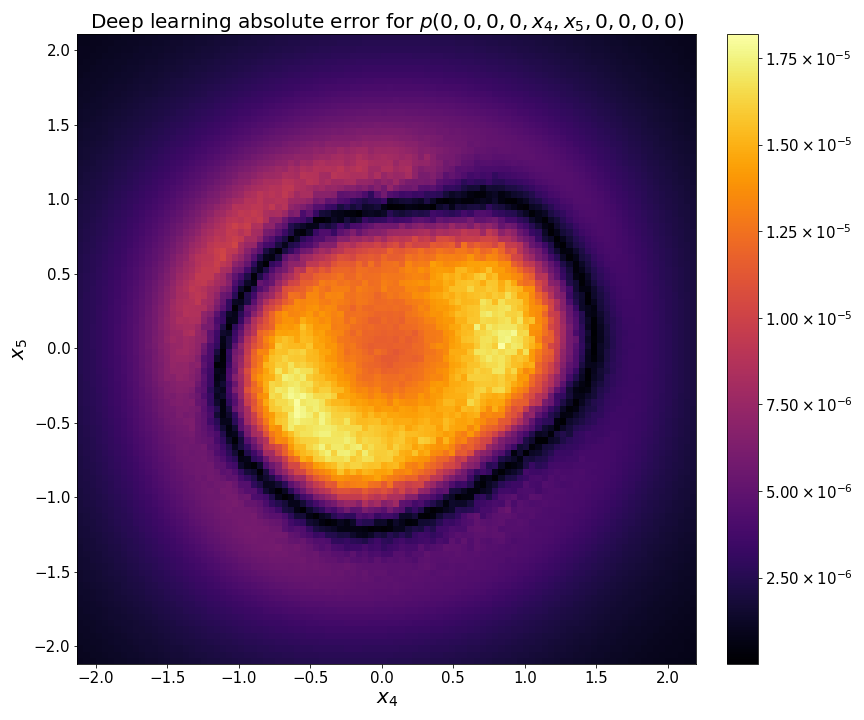
\includegraphics[scale=0.32]{steady-plots/10D-error.png}
\caption{Absolute error in the learned solution for the 10D ring system}
    \label{fig:10D-error}
\end{figure}

    

\subsection{Noisy Lorenz-63 system} Figure~\ref{fig:L63-steady} shows the results for the L63 system for $\Omega_I = [-30, 30]\times[-40, 40]\times[0, 70]$ and $E=10^6$. For ease of visualization the solutions have been normalized and in each row one of the dimensions has been integrated over the relevant interval to produce 2D marginals. In order to integrate out one dimension we use a composite Gauss-Legendre quadrature rule. We subdivide the relevant interval into 240 subintervals and use 10-point Gauss-Legendre rule to compute the integral over every subinterval. Note that since $n_\theta$ is a smooth function, our integrand is always a smooth function. The largest possible subinterval is of length $\frac{40-(-40)}{240}=\frac{1}{3}$ so assuming absolute value of the $20$-th derivative of the integrand is upper-bounded by $M$ everywhere, the integration error on each subinterval is upper-bounded by $\frac{2M}{20!}\left(\frac{1}{6}\right)^{20}\le2.25M\times10^{-34}$, see appendix~\ref{ssec-error-GL} for more details on this estimate. To produce the Monte Carlo solution, SDE trajectories were generated till time 10 with time-steps of $10^{-2}$. 
Since Monte Carlo produces lower-accuracy solutions even in lower dimensions as we saw in section~\ref{sssec-MC-comparison} and an analytic solution is unavailable in this case, we refrain from producing error plots.

\begin{figure}[!ht]
    \centering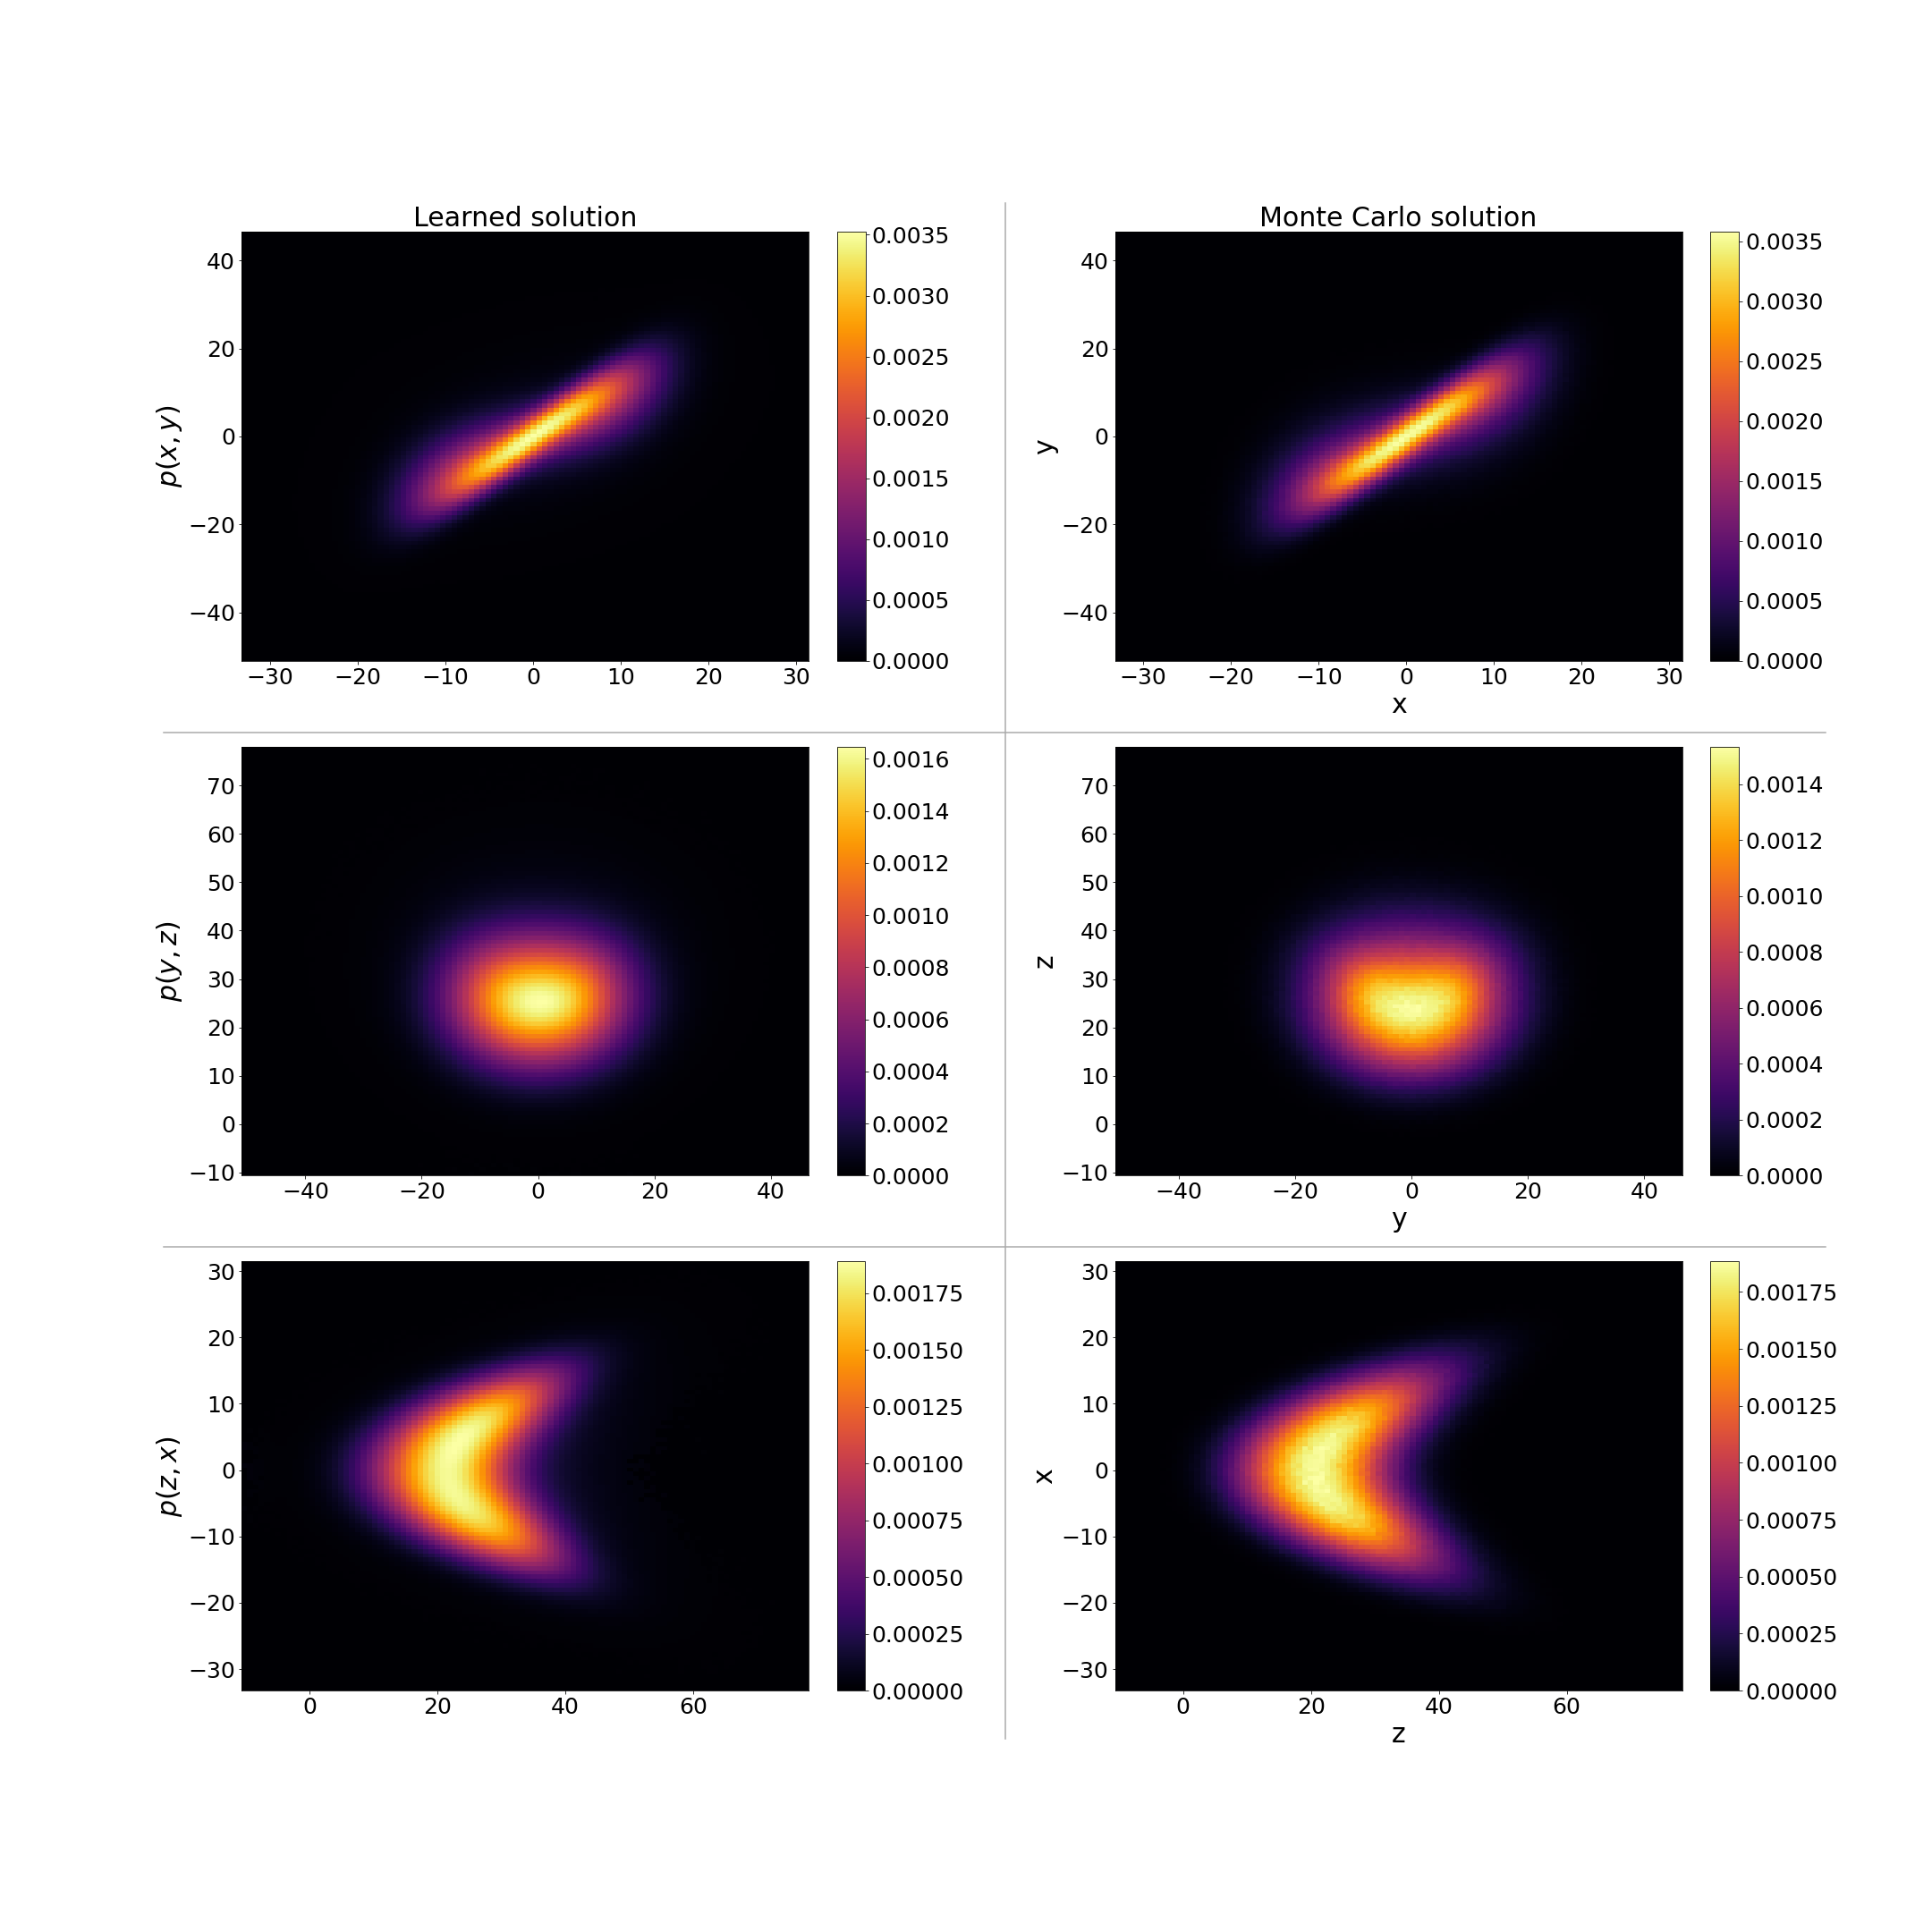
\includegraphics[scale=0.21]{steady-plots/L63-steady.png}  \caption{Solutions for the noisy Lorenz-63 system}
    \label{fig:L63-steady}
\end{figure}

\subsection{Noisy Thomas system}
Figure~\ref{fig:Thomas-steady} shows the results for the Thomas system for $\Omega_I = [-10, 10]^3$ and $E=4\times10^5$. Due to the inherent symmetry of this problem it suffices to compute only the 2D marginal $p(x, y)$. To integrate out the $z$ dimension we use 8-point composite Gauss-Legendre quadrature rule with $165$ subintervals. Assuming absolute value of the $16$-th derivative of the integrand is upper-bounded by $M$ everywhere, the integration error on each subinterval is upper-bounded by $\frac{2M}{16!}\left(\frac{10}{165}\right)^{16}\le3.17M\times10^{-33}$, see appendix~\ref{ssec-error-GL} for more details on this error estimate. To produce the Monte Carlo solution, SDE trajectories were generated till time 10 with time-steps of $10^{-2}$. Even though we have solved a lower dimensional problem here, Thomas system turns out to be the \textit{easiest} i.e. algorithm~\ref{algo:steady} converges faster for this system compared to the other ones as we will see in the next section.
\begin{figure}[!htp]
    \centering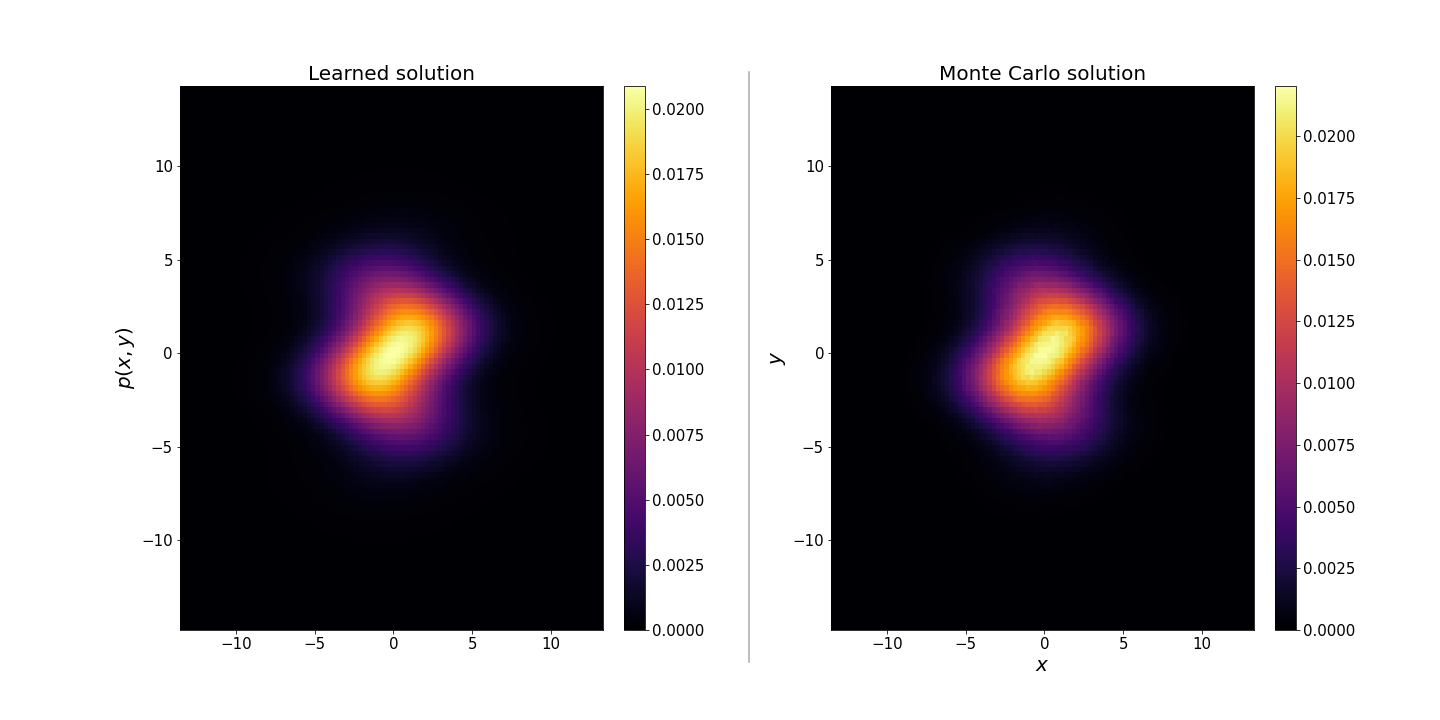
\includegraphics[scale=0.32]{steady-plots/Thomas-steady.png}
    \caption{Solutions for the noisy Thomas system}
    \label{fig:Thomas-steady}
\end{figure}
\subsection{Dimension dependence} In this section we explore the dimension dependence of algorithm~\ref{algo:steady}.
In the left panel of figure~\ref{fig:time-loss} we have plotted the loss given by \eqref{eq:def-steady-loss} against training iterations for all the of the systems above in a semi-log manner starting from iteration $100$. We often encounter spikes in the loss curve for the following reasons
\begin{itemize}
    \item the loss curves are single realizations of algorithm~\ref{algo:steady} instead of being an average
    \item we resample the domain every $10$ iterations and if the new points belong to a previously unexplored region in $\Omega_I$, the loss might increase.
\end{itemize}
But the general trend of loss diminishing with iterations is true for every system. We also see that loss is system-dependent and the \textit{hardness} of these problems or how quickly algorithm~\ref{algo:steady} converges depends on the nature of $\mu$ as much as the dimension. This is easily seen by noting that the two 3D systems sandwich the 2D and the 4D ring systems in the left panel of figure~\ref{fig:time-loss}. The loss for Thomas system drops very quickly compared to the rest of the systems due to the simplicity and global Lipschitzness of the corresponding drift function. We also see from the right panel of figure~\ref{fig:time-loss} that time taken per training iteration grows near-linearly with dimension. Since it is hard to estimate the amount of iterations to run before the loss drops below a pre-determined level, we refrain from plotting the total runtime of algorithm~\ref{algo:steady} against dimension. But it's interesting to note that the number of total training iterations $E$ varies from $4\times10^5$ to $4.6\times10^6$ across all the problems. Since the data shown in the right panel of figure~\ref{fig:time-loss} is very much hardware dependent, at this point we disclose that all of the experiments were done using the cloud service provided by Google Colab. This service automatically assigns runtimes to different hardware depending on availability at the time of computation which might explain why the 8D and 10D ring systems take nearly the same amount of time per iteration in figure~\ref{fig:time-loss}.
\begin{figure}[!ht]
    \centering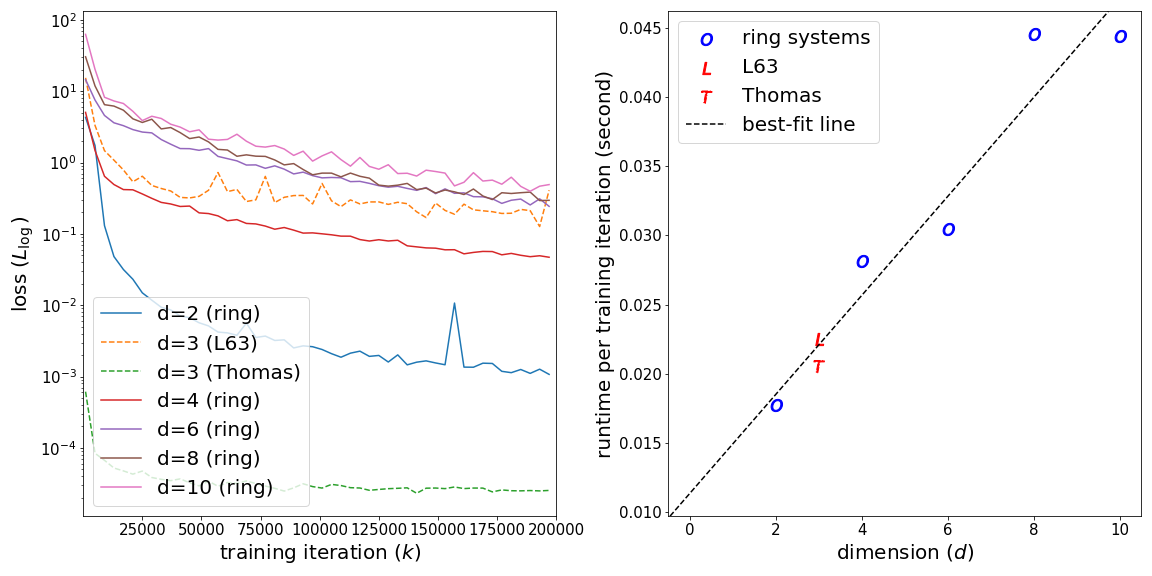
\includegraphics[scale=0.4]{steady-plots/loss-time.png}
    \caption{Left panel: Loss vs training iteration starting from iteration $100$. Right panel: time taken per training iteration vs dimension.}
    \label{fig:time-loss}
\end{figure}
\subsection{Comparison of loss and distance from truth} In this section we explore the relationship between the loss given by \eqref{eq:def-steady-loss} and the distance from truth. In spite of being structurally completely different, both are measures of goodness for a computed solution. In most cases we only have access to the loss and therefore it is an important question if going a decreasing loss implies getting closer to the truth for algorithm~\ref{algo:steady}. We define the distance of the learned zero from the true solution as follows,
\begin{align}
    \|g\|_*\stackrel{\rm def}{=}\sup_{\mathbf x\in\Omega_I} |cg(\mathbf x) - p^{\rm true}(\mathbf x)|\label{eq:def-sup-norm}, \qquad c\int_{\mathbb R^d}g=1
\end{align}
where $p^{\rm true}$ is the true solution to \eqref{eq:SFPE-0}. \eqref{eq:def-sup-norm} is not easy to compute in arbitrary dimensions but can be computed for the 2D ring system without too much effort since $p^{\rm true}$ is known and the problem is low-dimensional. Figure~\ref{fig:dist-loss} shows the results for the 2D ring system. The right panel of figure~\ref{fig:dist-loss} shows that loss and distance from truth are strongly correlated for algorithm~\ref{algo:steady}. Moreover, asymptotically for small values of the loss function they are linearly related with a Pearson correlation coefficient $R=0.98$ as can be seen from the inset in the right panel which depicts the data from training iteration 10000 to 50000. The best-fit line is also shown in the inset. On the left panel we see that the distance from truth monotonically decreases with training iteration and is extremely well approximated by a curve of the form $a_0e^{-a_1k}+a_2$. Both panels contain data from training iteration 5000 to 50000. We omit the first few iterations to filter out the effects of the random initialization of the trainable parameters. Figure~\ref{fig:dist-loss} serves as a good justification for algorithm~\ref{algo:steady} since it shows that minimizing the loss is akin to getting closer to a true non-trivial zero of $\mathcal L$.
 
\begin{figure}[!ht]
    \centering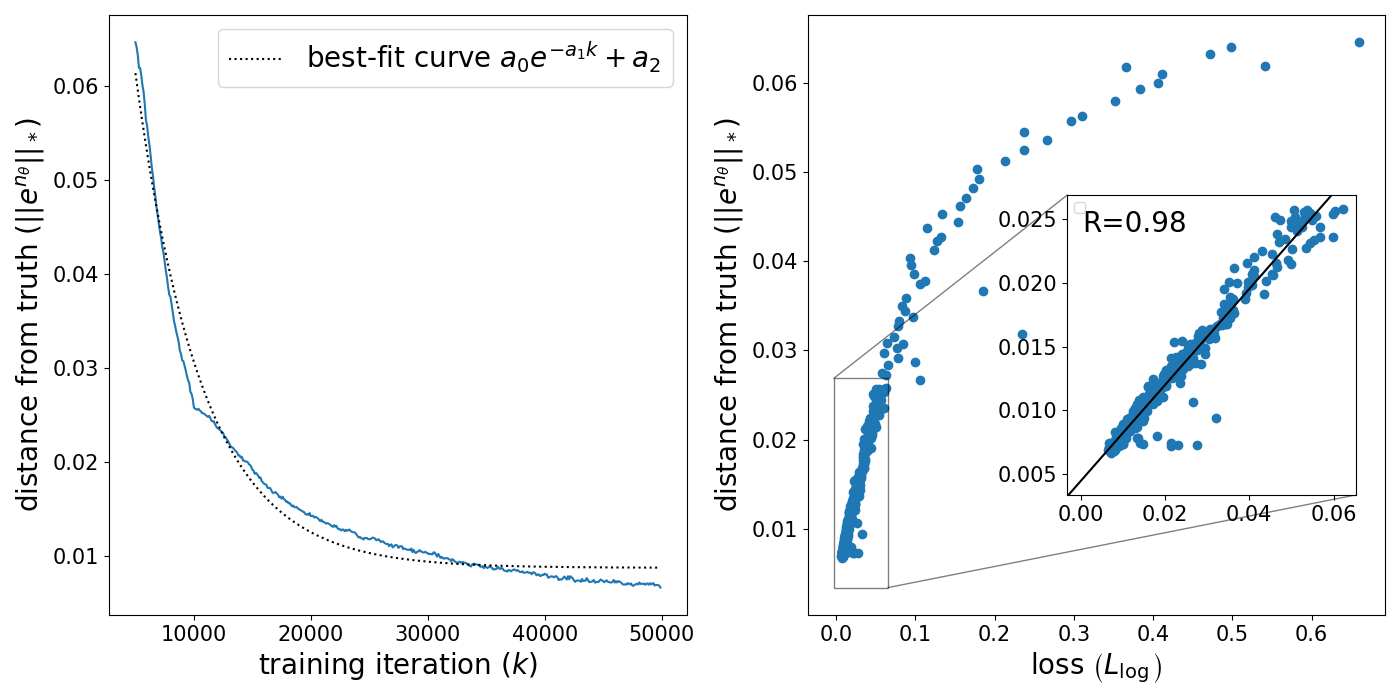
\includegraphics[scale=0.4]{steady-plots/2D-distance.png}
    \caption{Left panel: Distance from truth vs training iteration every 100 iterations, starting from iteration 5000 and ending at iteration 50000 for the 2D ring system. Right panel: Scatter plot for loss vs distance from truth for the 2D ring system. The inset shows that asymptotically loss and the distance from the truth are linearly related. The inset depicts the data from training iteration $10000$ to $50000$.}
    \label{fig:dist-loss}
\end{figure}